% Notes and solutions


% -------------------------------------------------
% Package imports
% -------------------------------------------------
\documentclass[12pt, a4paper]{article}
\usepackage[utf8]{inputenc}% Input encoding
\usepackage[english]{babel}% Set language to english
\usepackage{graphicx}% For importing graphics
\usepackage{amsthm, amsfonts, amssymb, bm}% All the AMS packages
\usepackage{mathtools}% Fixes a few AMS bugs
\usepackage[expansion=false]{microtype}% Fixes to make typography better
\usepackage{hyperref}% For \href{URL}{text}
\usepackage{fancyhdr}% For fancy headers
\usepackage[sharp]{easylist}% Easy nested lists
\usepackage{parskip}% Web-like paragraphs
\usepackage{multicol}% For multiple columns
\usepackage{tikz-cd}% For diagrams
\usepackage{microtype}
\usepackage{listings}% To include source-code
\usepackage[margin = 2.5cm, includehead]{geometry}% May be used to set margins
\usepackage{nicefrac}% Enables \nicefrac{nom}{denom}
%\usepackage[sc]{mathpazo}% A nice font, alternative to CM

% -------------------------------------------------
% Package setup
% -------------------------------------------------

\newcommand{\Title}{Learning Machine Learning}
\newcommand{\Subtitle}{A summary of main ideas and concepts}
\newcommand{\Author}{tommyod}
\newcommand{\listSpace}{-0.5em}% Global list space

\title{\Title}
\author{\Author}

% Shortcuts for sets and other stuff in mathematics
\newcommand{\Q}{\mathbb{Q}}
\newcommand{\R}{\mathbb{R}}
\newcommand{\C}{\mathbb{C}}
\newcommand{\D}{\mathcal{D}}
\newcommand{\Reg}{\mathcal{R}}
\newcommand{\Class}{\mathcal{C}}
\newcommand{\Z}{\mathbb{Z}}
\renewcommand{\sf}[1]{\mathsf{#1}}
\newcommand{\vect}[1]{\bm{#1}}
\newcommand{\norm}[1]{\left\lVert#1\right\rVert}
\newcommand{\abs}[1]{\left\lvert#1\right\rvert}

% Shortcuts for probability distributions
\DeclareMathOperator{\N}{\mathcal{N}}
\DeclareMathOperator{\Bern}{\operatorname{Bern}}
\DeclareMathOperator{\Beta}{\operatorname{Beta}}
\DeclareMathOperator{\Bin}{\operatorname{Bin}}
\DeclareMathOperator{\St}{\operatorname{St}}
\DeclareMathOperator{\U}{\operatorname{U}}
\DeclareMathOperator{\KL}{\operatorname{KL}}

% Shortcuts for statistical operators
\DeclareMathOperator{\E}{\mathbb{E}}
\DeclareMathOperator{\var}{\operatorname{var}}
\DeclareMathOperator{\cov}{\operatorname{cov}}
\DeclareMathOperator{\SD}{\operatorname{SD}}
\renewcommand{\H}{\operatorname{H}}



% Change the section command to inluce lines, save space, etc.
%\usepackage{titlesec}
%\titlespacing\subsection{0pt}{6pt plus 4pt minus 2pt}{-0.8em plus 4pt minus 2pt}
%\titlespacing\paragraph{0pt}{6pt plus 4pt minus 2pt}{8pt plus 4pt minus 2pt}
%\titleformat{\section}
%{\normalfont\Large\bfseries}{\thesection}{0em}{$\vartriangleright$ }[{\titlerule[1.2pt]}]

% -------------------------------------------------
% Document start
% -------------------------------------------------
\begin{document}
	
\maketitle
\begin{abstract}
This document contains some notes and solutions to the book ``Pattern Classification'' by Duda et al.
\end{abstract}

\tableofcontents

\section{Notes from ``Pattern Recognition''}

\section{Solutions to ``Pattern Recognition''}

\subsection{Bayesian Decision Theory}

\subsubsection*{Problem 2.6}
\begin{easylist}[enumerate]
\ListProperties(Space=\listSpace, Space*=\listSpace, Numbers1=l, FinalMark1={)})
# We want the probability of choosing action $\alpha_2$ to be smaller than, or equal to, $E_1$, given that the true state of nature is $\omega_1$.
Let's assume that $\mu_1 < \mu_2$ and that the decision threshold is $x^*$, so we decide $\alpha_2$ if $x > x^*$.
We then have
\begin{align*}
	P(\alpha_2 | \omega_1) &\leq E_1 \\
	p(x > x^* | \omega_1) &\leq E_1 \\
	\left[1 - \int_{0}^{x^*} p(x | \omega_1)  \, dx \right] &\leq E_1
\end{align*}
We let $\Phi: \R \to \left[0, 1\right]$ denote the cumulative Gaussian distribution, and $\Phi^{-1}: \left[0, 1\right] \to \R$ it's inverse function.
Making use of $\Phi$ we write
\begin{align*}
1 - \Phi \left( \frac{x^* - \mu_1}{\sigma_1} \right) &\leq E_1 \\
x^* \geq \mu_1 + \sigma_1 \Phi^{-1} \left(1 - E_1 \right).
\end{align*}
If the desired error is close to zero, then $x^*$ goes to positive infinity.
If the desired error is close to one, then $x^*$ goes to negative infinity.

# The error rate for classifying $\omega_2$ as $\omega_1$ is
\begin{equation*}
	P(\alpha_1 | \omega_2) = 	p(x \leq x^* | \omega_2) = \int_{0}^{x^*} p(x| \omega_2) \, dx 
	= 
	\Phi \left(  \frac{x^* - \mu_2}{\sigma_2}  \right).
\end{equation*}
Making use of $x^*$ from the previous problem, we obtain
\begin{equation*}
 \Phi \left(  \frac{ \mu_1 + \sigma_1 \Phi^{-1} \left(1 - E_1 \right) - \mu_2}{\sigma_2}  \right) 
 =
\Phi \left(  \frac{\mu_1 - \mu_2}{\sigma_2} + \frac{\sigma_1}{\sigma_2}  \Phi^{-1} \left(1 - E_1 \right) \right).
\end{equation*}
# The overall error rate becomes
\begin{align*}
	P(\text{error}) &= P(\alpha_1, \omega_2) + P(\alpha_2, \omega_1) \\
	&= P(\alpha_1 | \omega_2) P(\omega_2) + P(\alpha_2| \omega_1) P(\omega_1) \\
	&= \frac{1}{2} \left[  P(\alpha_1 | \omega_2) +  P(\alpha_2| \omega_1) \right] \\
	&= \frac{1}{2} \left[ E_1 +  \Phi \left(  \frac{\mu_1 - \mu_2}{\sigma_2} + \frac{\sigma_1}{\sigma_2}  \Phi^{-1} \left(1 - E_1 \right) \right) \right].
\end{align*}
In the last equality we used the results from the previous problems.

# We substitute the given values into the equations, and obtain $x^* \approx 0.6449$. The total error rate is $P(\text{error}) \approx 0.2056$.
# The Bayes error rate, as a function of $x^*$, is given by
\begin{align*}
	P(\text{error}) = P(\alpha_2 | \omega_1) P(\omega_1) + P(\alpha_1| \omega_2) P(\omega_2) \\
	= \frac{1}{2} \left[ p( x > x^*| \omega_1)  + p( x < x^* | \omega_2) \right]   \\
	= \frac{1}{2} \left[ \left( 1 - \Phi \left( \frac{x^* - \mu_1}{\sigma_1}\right)\right) +  \Phi \left( \frac{x^* - \mu_2}{\sigma_2}\right)  \right]
\end{align*}
The Bayes error rate is depicted in Figure \ref{fig:duda_ch2_prob6}.

\begin{figure}[ht!]
\centering
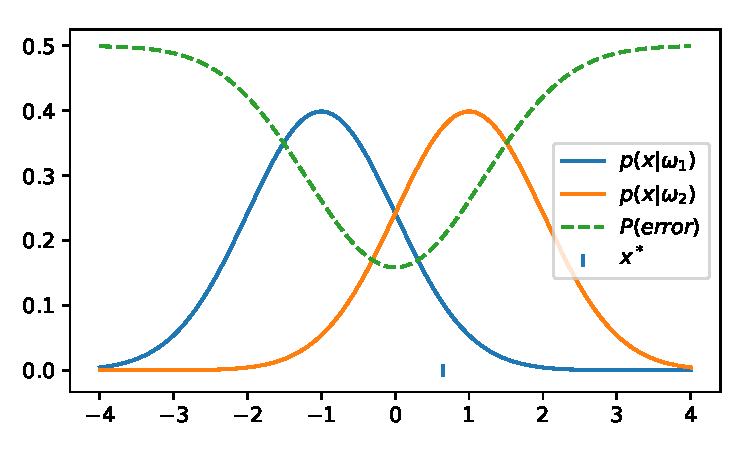
\includegraphics[width=0.5\linewidth]{figs/duda_ch2_prob6}
\caption{Graf accompanying problem 2.6.}
\label{fig:duda_ch2_prob6}
\end{figure}


\end{easylist}

\subsubsection*{Problem 2.12}
\begin{easylist}[enumerate]
\ListProperties(Space=\listSpace, Space*=\listSpace, Numbers1=l, FinalMark1={)})
# The key observation is that the maximal value $P(\omega_{\text{max}} | \vect{x} )$ is greater than, or equal to, the average. Therefore we obtain
\begin{equation*}
	P(\omega_{\text{max}} | \vect{x} ) \geq \frac{1}{c} \sum_{i=1}^{c} P(\omega_i | \vect{x}) = \frac{1}{c},
\end{equation*}
where the last equality is due to probabilities summing to unity.
# The minimum error rate is achieved by choosing $\omega_{\text{max}}$, the most likely state of nature. 
The average probability of error over the data space is therefore the probability that $\omega_{\text{max}}$ is \emph{not} the true state of nature for a given $\vect{x}$, that is:
\begin{equation*}
	P(\text{error}) = \E_x \left[ 1 - P(\omega_{\text{max}} | \vect{x} ) \right] = 1 - \int P(\omega_{\text{max}} | \vect{x} ) p(\vect{x}) \, d \vect{x}.
\end{equation*}

# We see that
\begin{equation*}
	P(\text{error}) = 1 - \int P(\omega_{\text{max}} | \vect{x} ) p(\vect{x}) \, d \vect{x} \leq 1 - \int \frac{1}{c} p(\vect{x}) \, d \vect{x} = 1 - \frac{1}{c} = \frac{c-1}{c},
\end{equation*}
where we used $\int p(\vect{x}) \, d \vect{x} = 1$.


# A situation where $P(\text{error}) = (c-1)/c$ arises when $P(\omega_i) = 1/c$ for every $i$. Then the maximum value is equal to the average value, and the inequality in problem a) becomes an equality.
\end{easylist}


\subsubsection*{Problem 2.19}
\begin{easylist}[enumerate]
\ListProperties(Space=\listSpace, Space*=\listSpace, Numbers1=l, FinalMark1={)})
# The entropy is given by $\H\left[p(x)\right] = - \int p(x) \ln p(x) \, dx$.
The optimization problem gives the synthetic function
\begin{align*}
	H_s = - \int p(x) \ln p(x) \, dx + \sum_{k=1} ^{q} \lambda_k \left( \int b_k(x) p(x) \, dx - a_k \right),
\end{align*}
and since a probability density function has $\int p(x) \, dx = 1$ we add an additional constraint for $k=0$ with $b_0(x) = 1$ and $a_k = 1$.
Collecting terms we obtain
\begin{align*}
H_s &= - \int p(x) \ln p(x) \, dx + \sum_{k=0} ^{q} \lambda_k  \int b_k(x) p(x) \, dx - \sum_{k=0} ^{q} \lambda_k a_k  \\
&= - \int p(x) 
\left[ \ln p(x) - \sum_{k=0} ^{q} \lambda_k b_k(x) \right] \, dx - \sum_{k=0} ^{q} \lambda_k a_k ,
\end{align*}
which is what we were asked to show.
# Differentiating the equation above with respect to $p(x)$ and equating it to zero we obtain
\begin{equation*}
	- \int \left(  1 \left[ \ln p(x) - \sum_{k=0} ^{q} \lambda_k b_k(x) \right] + p(x) \left[ \frac{1}{p(x)} \right] \right) \, dx = 0.
\end{equation*}
This integral is zero if the integrand is zero for every $x$, so we require that
\begin{equation*}
	 \ln p(x) - \sum_{k=0} ^{q} \lambda_k b_k(x) + 1 = 0,
\end{equation*}
and solving this equation for $p(x)$ gives the desired answer.
\end{easylist}

\subsubsection*{Problem 2.21}
We are asked to compute the entropy of the (1) Gaussian distribution, (2) triangle distribution and (3) uniform distribution. 
Every p.d.f has $\mu = 0$ and standard deviation $\sigma$, and we must write every p.d.f parameterized using $\sigma$.
\paragraph{Gaussian} We use the definition $\H\left[p(x)\right] = - \int p(x) \ln p(x) \, dx$ to compute  
\begin{equation*}
	\H\left[p(x)\right] = 
	- \int \frac{1}{\sqrt{2 \pi} \sigma} 
	\exp \left( - \frac{1}{2} \frac{x^2}{\sigma^2} \right) 
	\left[ \ln \left( \frac{1}{\sqrt{2 \pi} \sigma } \right) - \frac{1}{2} \frac{x^2}{\sigma^2} \right] \, dx.
\end{equation*}
Let us denote $K = \frac{1}{\sqrt{2 \pi} \sigma} $ to simplify notation. We obtain
\begin{align*}
	- \int & K
	\exp \left( - \frac{1}{2} \frac{x^2}{\sigma^2} \right) 
	\left[ \ln K - \frac{1}{2} \frac{x^2}{\sigma^2} \right] \, dx = \\
	- K \ln K \int & 
	\exp \left( - \frac{1}{2} \frac{x^2}{\sigma^2} \right) \, dx + K \int  \frac{1}{2} \frac{x^2}{\sigma^2} \exp \left( - \frac{1}{2} \frac{x^2}{\sigma^2} \right)  \, dx
\end{align*}
The first term is simply negative $\ln K$, since it's the normal distribution with an additional factor $-\ln K$.
The second term is not as straightforward.
We change variables to $y = x / \left( \sqrt{2} \sigma \right)$, and write it as
\begin{equation*}
	K \int  y^2 \exp \left( - y^2 \right) \sqrt{2} \sigma \, dy,
\end{equation*}
which can be solved by using the following observation (from integration by parts)
\begin{equation*}
	\int 1 e^{-x^2} \, dx = \underbrace{\left. x e^{-x^2} \right|}_{0\text{ at } \pm \infty} - \int x (-2x) e^{-x^2} \, dx.
\end{equation*}
Using the above equation in reverse, we integrate as follows:
\begin{equation*}
	K \sqrt{2} \sigma \int  y^2 \exp \left( - y^2 \right)  \, dy = 	K \sqrt{2} \sigma \frac{1}{2}\int  \exp \left( - y^2 \right)  \, dy = K \sqrt{2} \sigma \frac{1}{2} \sqrt{\pi} = \frac{1}{2}
\end{equation*}
To recap, the first integral evaluated to $- \ln K$, and the second evaluated to $\frac{1}{2}$.
The entropy of the Gaussian is therefore $1/2 + \ln \sqrt{2 \pi } \sigma$.

\paragraph{Triangle}
The triangle distribution may be written in the form
\begin{equation*}
	f(x) = \begin{cases}
	h - \frac{hx}{b} &\quad \text{ if } \abs{x} < b\\
	0 &\quad \text{ if } \abs{x} \geq b,
	\end{cases}
\end{equation*}
where $h$ is the height and $b$ is the width to the left of, and to the right of, $x=0$.

Since the integral must evaluate to unity, we impose $hb = 1$ and obtain $f(x;b) = \frac{1}{b} \left( 1- \frac{x}{b}\right)$.
We wish to parameterize the triangle distribution using the standard deviation $\sigma$ instead of width $b$.
We can use $\var(X) = \E(X^2) - \E(X)^2$ to find the variance, since in this case $\E(X)^2 = \mu^2 = 0$ since the function is centered on $x=0$.
Computing $\E(X^2)$ yields $b^2 / 6$, so $b^2 = 6 \sigma^2$.
The revised triangle distribution then becomes
\begin{equation*}
f(x; \sigma) = \begin{cases}
\frac{1}{\sqrt{6} \sigma} \left(1 - \frac{x}{\sqrt{6} \sigma}\right) &\quad \text{ if } \abs{x} < \sqrt{6} \sigma \\
0 &\quad \text{ if } \abs{x} \geq \sqrt{6} \sigma .
\end{cases}
\end{equation*}
We set $k = \frac{1}{\sqrt{6} \sigma}$ to ease notation.
Due to symmetry, we compute the entropy as 
\begin{equation*}
	\H\left[f(x; \sigma)\right] = - 2 \int_{0}^{\sqrt{6} \sigma} k \left(1 - kx\right) \ln \left( k \left(1 - k x \right) \right) \, dx.
\end{equation*}
Changing variables to $y = 1 - kx$ we obtain
\begin{align*}
& - 2 \int_{x=0}^{x=\sqrt{6} \sigma} k y  \left( \ln k + \ln y \right) \, dx = - 2 \int_{y = 1}^{y = 0} k y  \left( \ln k + \ln y \right) \left(\frac{1}{-k}\right) \, dy \\
& - 2 \int_{0}^{1} y \left( \ln k + \ln y \right) dy = - 2 \int_{0}^{1} y \ln k \, dy - 2 \int_{0}^{1} y  \ln y \, dy = -2 \left( \ln k - \frac{1}{4}\right),
\end{align*}
where the last integral can be evaluated using integration by parts.
The entropy of the triangle distribution turns out to be $1/2 + \ln \sqrt{6} \sigma$.

\paragraph{Uniform}
Using the same logic as with the triangle distribution to normalize a uniform distribution, and then parameterizing by $\sigma$, we obtain
\begin{equation*}
u(x; \sigma) =
\left\{\!\begin{aligned}
\frac{1}{2b} &\quad \text{ if } \abs{x} < b \\
0 &\quad \text{ if } \abs{x} \geq b 
\end{aligned}\right\}
= 
\left\{\!\begin{aligned}
\frac{1}{2\sqrt{3}\sigma} &\quad \text{ if } \abs{x} <\sqrt{3}\sigma \\
0 &\quad \text{ if } \abs{x} \geq \sqrt{3}\sigma.
\end{aligned}\right.
\end{equation*}
Computing the entropy is easier than in the case of the Gaussian and the triangle distribution, we simply evaluate the integral as
\begin{equation*}
\H\left[p(x)\right] =2  \int_0^{\sqrt{3} \sigma} \frac{1}{2\sqrt{3}\sigma} \ln \frac{1}{2\sqrt{3}\sigma}  \, dx = \ln 2 \sqrt{3} \sigma.
\end{equation*}.

Let's briefly compare the results of our computations as follows:
\begin{align*}
	H_\text{Gaussian}(\sigma) &= 1/2 + \ln \sqrt{2 \pi } \sigma = \frac{1}{2} + \ln \sqrt{2\pi}  + \ln \sigma \approx 1.4189 + \ln \sigma \\
	H_\text{Triangle}(\sigma) &= 1/2 + \ln \sqrt{6} \sigma = \frac{1}{2} + \ln \sqrt{6} + \ln \sigma \approx 1.3959 + \ln \sigma \\
	H_\text{Uniform}(\sigma) &= \ln 2 \sqrt{3} \sigma = 0 + \ln 2 \sqrt{3} + \ln \sigma \approx 1.2425 + \ln \sigma
\end{align*}
This verifies that out of the three distributions, the Gaussian has the maximal entropy.
This was expected, since the Gaussian maximizes the entropy over \emph{any} continuous p.d.f. having a prescribed mean and variance.



\subsubsection*{Problem 2.23}
\begin{easylist}[enumerate]
\ListProperties(Space=\listSpace, Space*=\listSpace, Numbers1=l, FinalMark1={)})
# To solve this problem, we need to find the inverse matrix, the determinant, and $\vect{w} = \vect{x} - \vect{\mu}$.
\begin{equation*}
	\vect{\Sigma}^{-1} = \frac{1}{21}\begin{pmatrix}
	1 & 0 & 0 \\
	0 & 5 & -2 \\
	0 & -2 & 5 \\
	\end{pmatrix}
	\quad
	\det \vect{\Sigma} = 21
	\quad
	\vect{w} = \vect{x} - \vect{\mu} = 
	\begin{pmatrix}
	-0.5 \\
	-2 \\
	-1
	\end{pmatrix}
\end{equation*}
The number of dimension $d$ is 3.
The solution is
\begin{equation*}
	p(\vect{x}) = \frac{1}{\left(2 \pi \right)^\frac{3}{2} 21^{\frac{1}{2}}} \exp \left( -\frac{1}{2} \vect{w}^T \vect{\Sigma}^{-1} \vect{w}\right)
	= \frac{1}{\left(2 \pi \right)^\frac{3}{2} 21^{\frac{1}{2}}} \exp \left( -\frac{1}{2} \frac{1}{21} \frac{69}{4}\right).
\end{equation*}
# The eigenvectors of $\vect{\Sigma}$ are $\lambda_1 = 3$, $\lambda_1 = 7$ and $\lambda_1 = 21$.
The corresponding eigenvectors are
$\vect{v}_1 = (0, 1, -1)^T / \sqrt{2}$, 
$\vect{v}_2 = (0, 1, 1)^T / \sqrt{2}$ and 
$\vect{v}_3 = (1, 0, 0)^T$.
The whitening transformation is therefore given by
\begin{equation*}
	\vect{A}_w = \vect{\Phi} \vect{\Lambda}^{-1/2} = 
	\frac{1}{\sqrt{2}}
	\begin{pmatrix}
	0 & 0 & \sqrt{2} \\
	1 & 1 & 0 \\
	-1 & 1 & 0 \\
	\end{pmatrix}
	\begin{pmatrix}
	-\sqrt{3} & 0 & 0 \\
	0 & -\sqrt{7} & 0 \\
	0 & 0 & -\sqrt{21} 
	\end{pmatrix}.
\end{equation*}
The rest of the numerical computations are skipped.
# Skipped.
# Skipped.
# We are going to examine if the p.d.f is unchanged when vectors are transformed with $\vect{T}^T \vect{x}$ and matrices with $\vect{T}^T \vect{\Sigma} \vect{T}$.
Let's consider the term $\left(\vect{x} - \vect{\mu}\right)^T \vect{\Sigma}^{-1} \left(\vect{x} - \vect{\mu}\right)$ in the exponent first.
Substituting $\vect{x} \mapsto \vect{T}^T \vect{x}$,
$\vect{\mu} \mapsto \vect{T}^T \vect{\mu}$ and
$\vect{\Sigma} \mapsto \vect{T}^T \vect{\Sigma} \vect{T}$, we observe that
\begin{gather*}
	\left(\vect{T}^T\vect{x} - \vect{T}^T\vect{\mu}\right)^T
	 \left( \vect{\vect{T}^T\Sigma}\vect{T}  \right)^{-1}
	 \left(\vect{T}^T\vect{x} - \vect{T}^T\vect{\mu}\right) \\
	\left(\vect{T}^T\left(\vect{x} - \vect{\mu}\right)\right)^T
	 \left( \vect{\vect{T}^T\Sigma}\vect{T}  \right)^{-1}
	 \vect{T}^T\left(\vect{x} - \vect{\mu}\right) \\
	 \left(\vect{x} - \vect{\mu}\right)^T \vect{T}
	 \left( \vect{T}^T \vect{\Sigma}\vect{T}  \right)^{-1}
	 \vect{T}^T\left(\vect{x} - \vect{\mu}\right) \\
	 \left(\vect{x} - \vect{\mu}\right)^T \vect{T}
	 \vect{T}^{-1} \vect{\Sigma}^{-1}\vect{T}^{-T}
	 \vect{T}^T\left(\vect{x} - \vect{\mu}\right) \\
	 \left(\vect{x} - \vect{\mu}\right)^T 
	  \vect{\Sigma}^{-1}
	 \left(\vect{x} - \vect{\mu}\right),
\end{gather*}
where we have used $(\vect{A}\vect{B})^T = \vect{B}^T \vect{A}^T$ and $(\vect{A}\vect{B})^{-1} = \vect{B}^{-1} \vect{A}^{-1}$, which are basic facts from linear algebra.
The density remains proportional when applying a linear transformation, but not unscaled, since the proportionality term $\abs{\vect{\Sigma}}^{1/2}$ becomes $\abs{\vect{T}^T \vect{\Sigma} \vect{T}}^{1/2} = \abs{\vect{T}^T}^{1/2}  \abs{\vect{\Sigma} }^{1/2}  \abs{ \vect{T}}^{1/2} = \abs{\vect{T}} \abs{\vect{\Sigma} }^{1/2}$.

# Here we use the eigendecomposition of a symmetric matrix.
We assume that $\vect{\Sigma}$ is positive definite such that every eigenvalue is positive. 
We write $\vect{\Sigma} = \vect{\Phi} \vect{\Lambda} \vect{\Phi}^T$ and apply the whitening transformation.
\begin{equation*}
	\vect{\vect{A}_w}^T \vect{\Sigma} \vect{\vect{A}_w} = 
	\vect{\vect{A}_w}^T \vect{\Phi} \vect{\Lambda} \vect{\Phi}^T \vect{\vect{A}_w}  = 
	\left( \vect{\Phi} \vect{\Lambda}^{-1/2} \right)^T \vect{\Phi} \vect{\Lambda} \vect{\Phi}^T \left( \vect{\Phi} \vect{\Lambda}^{-1/2} \right)
\end{equation*}
The matrix $\vect{\Phi}$ is orthogonal, so it's transpose is the inverse.
Using this fact and proceeding, we obtain
\begin{equation*}
\left( \vect{\Phi} \vect{\Lambda}^{-1/2} \right)^T \vect{\Phi} \vect{\Lambda} \vect{\Phi}^T \left( \vect{\Phi} \vect{\Lambda}^{1/2} \right) = \left( \vect{\Lambda}^{-1/2} \right)^T \vect{\Lambda} \vect{\Lambda}^{-1/2} = \vect{\Lambda}^{-1/2} \vect{\Lambda} \vect{\Lambda}^{-1/2} = \vect{I},
\end{equation*}
so the covariance is proportional to the identity matrix, as we were tasked to show.
The normalization constant becomes $1$ , since the proportionality term becomes $\abs{\vect{T}} \abs{\vect{\Sigma} }^{1/2}$ under the transformation, and 
\begin{equation*}
	\abs{\vect{T}} \abs{\vect{\Sigma} }^{1/2} = \abs{\vect{\Phi} \vect{\Lambda}^{-1/2}} \abs{\vect{\Sigma} }^{1/2} = \abs{\vect{\Phi} \vect{\Lambda}^{-1/2}} \abs{\vect{\Phi} \vect{\Lambda} \vect{\Phi}^T }^{1/2} = \abs{\vect{I}} = 1.
\end{equation*}
\end{easylist}

\subsubsection*{Problem 2.28}
\begin{easylist}[enumerate]
\ListProperties(Space=\listSpace, Space*=\listSpace, Numbers1=l, FinalMark1={)})
# We prove that if $p(x_i - \mu_i, x_j - \mu_j) = p(x_i - \mu_i) p(x_j - \mu_j)$, then $\sigma_{ij} = \E \left[ (x_i - \mu_i) (x_j - \mu_j)\right] = 0.$
With words: we prove that statistical independence implies zero covariance.
\begin{gather*}
	 \E \left[ (x_i - \mu_i) (x_j - \mu_j)\right] = \\
	 \iint p(x_i - \mu_i, x_j - \mu_j) (x_i - \mu_i) (x_j - \mu_j) \, dx_j dx_i = \\
	 \iint  p(x_i - \mu_i) p(x_j - \mu_j) (x_i - \mu_i) (x_j - \mu_j) \, dx_j dx_i \\
	 \int p(x_i - \mu_i) (x_i - \mu_i) \left( 
	 \int p(x_j - \mu_j) (x_j - \mu_j) \, dx_j
	   \right) \, dx_i
\end{gather*}
If the term in the parenthesis is identically zero, then $\sigma_{ij} = 0$.
This is indeed true, since we find that
\begin{equation*}
	\int p(x_j - \mu_j) (x_j - \mu_j) \, dx_j = \E \left[ (x_j - \mu_j)\right]
	= \E \left[x_j\right] -  \E \left[\mu_j\right] = \mu_j - \mu_j = 0.
\end{equation*}
# We wish to prove the converse of a) in the Gaussian case.
To achieve this, we must show that
$\sigma_{ij} = 0$ when $p(x_i - \mu_i, x_j - \mu_j) = p(x_i - \mu_i) p(x_j - \mu_j)$.
Let's simplify the notation to $x$ and $y$ instead of $x_i$ and $x_j$.
If $\sigma_{xy} = 0$, then the covariance matrix is a diagonal matrix $\vect{D} = \operatorname{diag}(\sigma_x^2, \sigma_y^2)$.
We write the probability $p(x_i - \mu_i, x_j - \mu_j)$ as $p(x,y)$, where the means $\mu_x$ and $\mu_y$ are both zero.
We write
\begin{gather*}
	p(x, y) = 
	\frac{1}{(2\pi)^{2/2} \sigma_x \sigma_y} \exp \left( - \frac{1}{2} \vect{x}^T \vect{D}^{-1} \vect{x} \right) = 
	\frac{1}{(2\pi)^{2/2} \sigma_x \sigma_y} \exp \left( - \frac{1}{2} \left( x^2 / \sigma_x^2 + y^2 / \sigma_y^2 \right) \right)  \\
	=  \frac{1}{(2\pi)^{1/2} \sigma_x} \exp \left( - \frac{1}{2} \left( x^2 / \sigma_x^2 \right) \right) 
	\frac{1}{(2\pi)^{1/2} \sigma_y} \exp \left( - \frac{1}{2} \left( y^2 / \sigma_y^2 \right) \right)
	= p(x) p(y).
\end{gather*}
This proves that when $\sigma_{xy} = 0$, the covariance matrix is diagonal, and the Gaussian factors into products and we have statistical independence.

# This problem asks us to find a counterexample of the above, i.e. an example showing that $\sigma_{xy} \nRightarrow p(x, y) = p(x) p(y)$.
The probability density function
\begin{equation*}
	p(x, y) = K \frac{1}{1 + x^2 + y^2}, \quad K^{-1} = \iint_{\R} \frac{1}{1 + x^2 + y^2} \, dx dy
\end{equation*}
achieves this.
The covariance is zero, since $\sigma_{xy} = \E \left[ (x - 0) (y - 0)\right] = \iint_{\R} \frac{x y}{1 + x^2 + y^2} \, dx dy = \iint_{\R} I(x, y) \, dx dy$ is zero because the integrand $I(x, y)$ is an odd function.

On the other hand, $p(x, y)$ does \emph{not} factor into $p(x) p(y)$.
We have proved that $\sigma_{xy} \nRightarrow p(x, y) = p(x) p(y)$ by finding a counterexample.
\end{easylist}
\subsubsection*{Problem 2.31}
\begin{easylist}[enumerate]
\ListProperties(Space=\listSpace, Space*=\listSpace, Numbers1=l, FinalMark1={)})
# We'll assume that $\mu_1 < \mu_2$.
Since $\sigma_1 = \sigma_2 = \sigma$, the minimum probability of error is achieved by setting the decision threshold to $x^* = (\mu_1 + \mu_2)/2$.
To follow the derivation below, it helps to draw the real line and two Gaussians.
The probability of error is then
\begin{align*}
	P_e &= P(x \in R_2, \omega_1) + P(x \in R_1, \omega_2) \\
	&= 
	P(x \in R_2 | \omega_1) P(\omega_1)  + P(x \in R_1 | \omega_2) P(\omega_2) \\&= 
	\int_{R_2} p(x | \omega_1) P(\omega_1) \, dx + \int_{R_1} p(x | \omega_2) P(\omega_2) \, dx
	 \\
	 &= \frac{1}{2}\left( \int_{x^*}^{\infty} p(x | \omega_1) \, dx + 
	 \int_{0}^{x^*} p(x | \omega_2) \, dx \right) = \int_{x =(\mu_1 + \mu_2)/2 }^{\infty} p(x | \omega_1) \, dx \\
	 &=
	 \int_{x =(\mu_1 + \mu_2)/2 }^{\infty} \frac{1}{\sqrt{2 \pi } \sigma} \exp\left( - \frac{1}{2} \frac{(x - \mu_1)^2}{\sigma^2}\right) \, dx.
\end{align*}
Changing variables to $u = (x - \mu_1) / \sigma$ and using $dx = \sigma \, du$ yields
\begin{equation*}
	P_e = \int_{u=a}^{\infty} \frac{1}{\sqrt{2 \pi }} \exp\left( -u^2 /\sigma^2 \right) \, du,
\end{equation*}
where $a = (x - \mu_1 )/\sigma = ((\mu_1 + \mu_2)/2 - \mu_1 )/\sigma =  (\mu_2 - \mu_1) / 2 \sigma$, as required.

# Using the inequality stated in the problem, it remains to show that
\begin{equation*}
	\lim_{a \to \infty} f(a) = \lim_{a \to \infty} \frac{1}{\sqrt{2 \pi} a} \exp\left( -a^2 /\sigma^2 \right) = 0.
\end{equation*}
This holds if the derivative is negative as $a \to \infty$, since then the function decreases as $a \to \infty$. The derivative of $f(a)$ is
\begin{equation*}
	f'(x) = -\exp\left( -a^2 / 2\right) \left( 1 - \frac{1}{a^2}\right),
\end{equation*}
which is negative as long as $\abs{a} \geq 1$.
Alternatively, we see that both factors in $f(a)$ go to zero as $a \to \infty$.
\end{easylist}

\subsubsection*{Problem 2.43}
\begin{easylist}[enumerate]
	\ListProperties(Space=\listSpace, Space*=\listSpace, Numbers1=l, FinalMark1={)})
	# $p_{ij}$ is the probability that the $i$'th entry in the vector $\vect{x}$ equals $1$, given a state of nature $\omega_j$.
	# We decide $\omega_j$ if $P(\omega_j | \vect{x})$ is greater than $P(\omega_k | \vect{x})$ for every $k \neq j$.
	\begin{equation*}
	P(\omega_j | \vect{x}) \propto p(  \vect{x} | \omega_j) P(\omega_j)
	\end{equation*}
	We use the fact that $p(  \vect{x} | \omega_j) = \prod_{i = 1}^{d} p(  x_i| \omega_j)$, which follows from the fact that the entries are statistically independent.
	Furthermore, we see that
	\begin{equation*}
	p(  x_i| \omega_j) = 
	\left\{\!\begin{aligned}
	p_{ij} &\quad \text{ if } x_i = 1 \\
	1 - p_{ij} &\quad \text{ if } x_i = 0 
	\end{aligned}\right\} = 
	p_{ij}^{x_i} \left( 1 - p_{ij}\right)^{ 1 - x_i}.
	\end{equation*}
	Now we take logarithms and  obtain
	\begin{align*}
	& \ln \left( \prod_{i = 1}^{d} p(  x_i| \omega_j) P(\omega_j) \right) =
	\sum_{i = 1}^{d} \ln p(  x_i| \omega_j)  + \ln P(\omega_j) \\
	& = \sum_{i = 1}^{d} \ln p_{ij}^{x_i} \left( 1 - p_{ij}\right)^{ 1 - x_i}  + \ln P(\omega_j) \\
	&
	= \sum_{i = 1}^{d} x_i \ln p_{ij} + (1 - x_i) \ln ( 1 - p_{ij})  + \ln P(\omega_j),
	\end{align*}
	which is easily arranged to correspond with the expression in the problem statement. 
	In summary we choose the class $\omega_j$ if the probability of that class given the data point exceeds the probability of every other class.
\end{easylist}




\subsection{Maximum-likelihood and Bayesian parameter estimation}

\subsubsection*{Problem 3.2}
\begin{easylist}[enumerate]
\ListProperties(Space=\listSpace, Space*=\listSpace, Numbers1=l, FinalMark1={)})
# The maximum likelihood estimate for $\theta$ is $\max_\theta p(x | \theta) = \max_\theta \prod_{i=1}^{n} p(x_i | \theta)$.
The probability $p(x_i | \theta)$ is given by the expression
\begin{equation*}
	p(x_i | \theta) = 
	\begin{dcases*}
	1/\theta & if $0 \leq x_i \leq \theta$ \\
	0 & if $ x_i > \theta$
	\end{dcases*}
\end{equation*}
The entire product $\prod_{i=1}^{n} p(x_i | \theta)$ is zero if any $x_i$ is larger than $\theta$, since then the corresponding factor is zero.
Thus $\theta$ must be larger than, or equal to, $\max_k x_k$.

On the other hand, the product equals $\frac{1}{\theta^n}$, and taking logarithms we obtain $-n \ln \theta$.
This function is maximized when $\theta$ is as small as possible.

The conclusion is that $\theta$ (1) must be $\geq \max_k x_k$ to avoid the likelihood being zero, and (2) as small as possible to maximize the likelihood.
Therefore we choose $\hat{\theta} = \max_k x_k = \max \D$.

# Skipping this plot. The explanation of why the other points are not needed is given in part a).
\end{easylist}

\subsubsection*{Problem 3.4}
The maximum likelihood estimate is $p( \D | \vect{\theta}) = \prod_{k = 1}^{n} p( \vect{x} | \vect{\theta}) = \prod_{k = 1}^{n} \prod_{i=1}^{d}
 \theta_{i}^{x_{ik}} \left( 1 - \theta_i \right)^{\left(  1 - x_{ik} \right)}$.
 The log likelihood $\ell(\vect{\theta})$ is $ \ln p( \D | \vect{\theta}) $, which becomes
 \begin{equation*}
 	\ell(\vect{\theta}) = \sum_{k = 1}^{n} \sum_{i=1}^{d}
 	x_{ik} \ln \theta_i + (1 - x_{ik}) \ln \left( 1 - \theta_i\right).
 \end{equation*}
Differentiating $\ell(\vect{\theta})$ with respect to component $\theta_i$, every term in the sum $\sum_{i=1}^{d}$ vanishes except the $i$'th.
We perform the differentiation and equate the result to zero, yielding
\begin{equation*}
	\frac{d \ell(\vect{\theta})}{\theta_i} = \sum_{k=1}^{n} \left[ \frac{x_{ik}}{\theta_i} + \frac{x_{ik} - 1}{1 - \theta_i} \right] =
	 \sum_{k=1}^{n} \left[ x_{ik} - \theta_i \right] = 0.
\end{equation*}
Solving this for $\theta_i$ yields $\theta_i = \frac{1}{n} \sum_{k=1}^{n} x_{ik}$, or in vector notation, $\vect{\theta} = \frac{1}{n} \sum_{k=1}^{n} \vect{x}_k$.
This is what the problem asked us to show.

\subsubsection*{Problem 3.6}
\begin{easylist}[enumerate]
	\ListProperties(Space=\listSpace, Space*=\listSpace, Numbers1=l, FinalMark1={)})
	# sdf
\end{easylist}

\subsubsection*{Problem 3.9}
\begin{easylist}[enumerate]
	\ListProperties(Space=\listSpace, Space*=\listSpace, Numbers1=l, FinalMark1={)})
	# sdf
\end{easylist}

\subsubsection*{Problem 3.15}
\begin{easylist}[enumerate]
	\ListProperties(Space=\listSpace, Space*=\listSpace, Numbers1=l, FinalMark1={)})
	# sdf
\end{easylist}

\subsubsection*{Problem 3.18}
\begin{easylist}[enumerate]
	\ListProperties(Space=\listSpace, Space*=\listSpace, Numbers1=l, FinalMark1={)})
	# sdf
\end{easylist}

\subsubsection*{Problem 3.23}
\begin{easylist}[enumerate]
	\ListProperties(Space=\listSpace, Space*=\listSpace, Numbers1=l, FinalMark1={)})
	# sdf
\end{easylist}

\subsubsection*{Problem 3.30}
\begin{easylist}[enumerate]
	\ListProperties(Space=\listSpace, Space*=\listSpace, Numbers1=l, FinalMark1={)})
	# sdf
\end{easylist}

\subsubsection*{Problem 3.31}
\begin{easylist}[enumerate]
	\ListProperties(Space=\listSpace, Space*=\listSpace, Numbers1=l, FinalMark1={)})
	# sdf
\end{easylist}

\subsubsection*{Problem 3.34}
\begin{easylist}[enumerate]
	\ListProperties(Space=\listSpace, Space*=\listSpace, Numbers1=l, FinalMark1={)})
	# sdf
\end{easylist}

\subsubsection*{Problem 3.41}
\begin{easylist}[enumerate]
	\ListProperties(Space=\listSpace, Space*=\listSpace, Numbers1=l, FinalMark1={)})
	# sdf
\end{easylist}

\subsubsection*{Problem 3.48}
\begin{easylist}[enumerate]
	\ListProperties(Space=\listSpace, Space*=\listSpace, Numbers1=l, FinalMark1={)})
	# sdf
\end{easylist}




\subsubsection*{TEST}
\begin{easylist}[enumerate]
\ListProperties(Space=\listSpace, Space*=\listSpace, Numbers1=l, FinalMark1={)})
# sdf
\end{easylist}





\end{document}
